% !TEX root = ../TSG_Administrator's_Guide_SV20.11_v1.0_EN.tex
%
\pdfbookmark[0]{Decryption}{Decryption}
\chapter*{\hypertarget{link:Decryption}{Decryption}}
\label{sec:decrypt}

Except firewall, TSG has a proxy which utilizes MITM (Man-in-the-middle) technologies and enables you to perform layer 4-7 advanced manipulation of network traffic. 
The Proxy is deployed in transparent mode; thus, no proxy settings on browser side. The proxy can decrypt and inspect traffic to control protocols and certificate verification. 
The proxy handles encrypted traffic according to your configured security settings. Traffic will be reconstructed according to the TCP/IP protocol stack with the original headers 
(source IP, source Port, destination IP, destination Port, Protocol, etc.) and decrypted payload. Decryption prevents malicious encrypted content from entering your network 
and sensitive content from leaving your network concealed as encrypted traffic. 
Enabling decryption need preparing the keys and certificates required, creating decryption profiles and configuring traffic mirror profile. 

{
\color{linkblue}
\hyperlink{link:Decryption Concepts}{> Decryption Concepts} \\
\hyperlink{link:Keys and Certificates}{> Keys and Certificates} \\
\hyperlink{link:Certificate Managements}{> Certificate Managements}\\
\hyperlink{link:Proxy Profiles}{> Proxy Profiles}\\
}
\clearpage

\pdfbookmark[1]{Decryption Concepts}{Decryption Concepts}
\section*{\hypertarget{link:Decryption Concepts}{Decryption Concepts}}
\label{sec:decrypt:concept}

The Secure Sockets Layer (SSL) and Transport Layer Security (TLS) encryption protocols secure traffic between two entities, such as a web server and a client. Without special instructions, SSL in this document refers to SSL/TLS. SSL encapsulate traffic, encrypting data so that it is meaningless to entities other than the client and server with the certificates to affirm trust between the devices and the keys to decode the data.


The proxy uses certificates and keys to decrypt traffic to plaintext, and then enforces security settings on the plaintext traffic. After decrypting and inspecting traffic, the proxy re-encrypts the plaintext traffic as it exits the proxy to ensure privacy and security.


SSL decryption requires certificates to establish the proxy as a trusted third party, and to establish trust between a client and a server to secure an SSL/TLS connection. You can also use certificates when excluding servers from SSL decryption for technical reasons (the site breaks decryption for reasons such as certificate pinning, unsupported ciphers, or mutual authentication).


You can integrate a hardware security module (HSM) with TSG to enable enhanced security for the private keys. 
To learn more about integrating an HSM, see \hyperlink{link:Manage Keys with a Hardware Security Module}{\color{linkblue}{Manage Keys with a Hardware Security Module}}.

\pdfbookmark[1]{Keys and Certificates}{Keys and Certificates}
\section*{\hypertarget{link:Keys and Certificates}{Keys and Certificates}}
\label{sec:decrypt:keys}

Keys are strings of numbers typically generated using a mathematical operation involving random numbers and large primes. Keys transform strings—such as passwords and shared secrets—from unencrypted plaintext to encrypted ciphertext and from encrypted ciphertext to unencrypted plaintext. Keys can be symmetric (the same key is used to encrypt and decrypt) or asymmetric (one key is used for encryption and a mathematically related key is used for decryption). Any system can generate a key.


X.509 certificates establish trust between a client and a server to establish an SSL connection. A client attempting to authenticate a server (or a server authenticating a client) knows the structure of the X.509 certificate and therefore knows how to extract identifying information about the server from fields within the certificate, such as the FQDN or IP address (called a common name or CN within the certificate) or the name of the organization, or user to which the certificate was issued. A certificate authority (CA) must issue all certificates. After the CA verifies a client or server, the CA issues the certificate and signs it with a private key.


When you decrypt traffic, a session between the client and the server is established only if the firewall trusts the CA that signed the server certificate. In order to establish trust, the firewall must have the server root CA certificate in its Trusted Certificate Authorities list and use the public key contained in that root CA certificate to verify the signature. The firewall then presents a copy of the server certificate for the client to authenticate. You can also configure the firewall to use an enterprise CA for SSL Proxy. If the firewall does not have the server root CA certificate in its Trusted Certificate Authorities list, the firewall will present a copy of the server certificate signed by the Forward Untrust certificate to the client. The Forward Untrust certificate ensures that clients are prompted with a certificate warning when attempting to access sites hosted by a server with untrusted certificates.


The change of the static expiration time for new generated certificates will not cause a service shutdown or other problems that negatively affect the decryption.


TSG allows you to delete installed certificates, including default certificate, change global and default certificate; 
but if the certificate is already referenced by a policy, TSG does not allow deleting it. You can modify the referenced certificate instead. 
For detailed information on certificates, see \hyperlink{link:Certificate Management}{\color{linkblue}{Certificate Management}}.

\pdfbookmark[1]{Certificate Managements}{Certificate Managements}
\section*{\hypertarget{link:Certificate Managements}{Certificate Managements}}
\label{sec:decrypt:certificate}

The digital certificates are used to ensure trust between parties in a secure communication session. Each certificate contains a cryptographic key to encrypt plaintext or decrypt ciphertext. Each certificate also includes a digital signature to authenticate the identity of the issuer. The issuer must be in the list of trusted certificate authorities (CAs) of the authenticating party.

\pdfbookmark[2]{Trusted Certificate Authorities}{Trusted Certificate Authorities}
\subsection*{\hypertarget{link:Trusted Certificate Authorities}{Trusted Certificate Authorities}}
\label{sec:decrypt:certificate:trusted}

TSG trusts the most common and trusted authorities (CAs) by default. These trusted certificate providers are responsible for issuing the certificates TSG requires to secure connections to the internet. The additional CAs you might want to add are trusted enterprise CAs that your organization requires. You can perform the following to import a certificate:

\begin{description}
    \item[STEP 1.]	Select \textbf{Settings} > \textbf{Certificate Managements} and select \textbf{Trusted Certificate Authorities} tab, Click \textbf{Import}.
    \item[STEP 2.]	Add a \textbf{Name}. The name is case-sensitive and can have up to 128 characters. It can use only letters, numbers, hyphens, and underscores.
    \item[STEP 3.]	Click \textbf{Please upload} and upload a PEM (base64-encoded) format file.
    \item[STEP 4.]	Click \textbf{OK}.    
\end{description}

Go back to Trusted Certificate Authorities tab, you can view detailed information about the CA you just created. 
To edit and delete CAs, find the item you want to edit or delete in the list. Click \textbf{Edit} or \textbf{Delete} at the top left. 
The system will periodically check whether the CA certificate has expired. 
If the CA certificate expires, the system will automatically set the status of the CA certificate to disable. 
To download it, you can click the cloud icon under \textbf{File}, and wait a few seconds for the file to be downloaded to your local folder. 
You can search CAs based on ID, Name, Issuer, Common Name and Certificate Fingerprint, or the combination. Enter search conditions in search bar and click search icon.

\pdfbookmark[2]{Decryption Keyrings}{Decryption Keyrings}
\subsection*{\hypertarget{link:Decryption Keyrings}{Decryption Keyrings}}
\label{sec:decrypt:certificate:keyring}

If your enterprise has its own public key infrastructure (PKI), you can import a certificate and private key into TSG from your enterprise certificate authority (CA). Enterprise CA certificates (unlike most certificates purchased from a trusted, third-party CA) can automatically issue CA certificates for applications such as SSL/TLS decryption.


Note that the built-in certificate with ID 1(\#1) means trusted certificate, and built-in certificate with ID 0(\#0) means untrusted certificate. You can add trusted certificate to TSG with two methods. One is local management with TSG interface through the following procedure; the other is integrate an external HSM device, the certificate will be saved to the HSM for specified website. For more details about HSM, see Manage Keys with a Hardware Security Module.


\notemark\textit{If the HSM is down, the firewall can process decryption for sites of HSM mode for which it has cached the response from the HSM, meanwhile the firewall will deploy default certificates (\#0 or \#1) for those un-cached sites of HSM mode.}


You can perform the following to Import a Certificate and Private Key:

\begin{description}
    \item[STEP 1.]	Select \textbf{Settings} > \textbf{Certificate Managements} and select \textbf{Decryption Keyrings} tab, Click \textbf{Create}
    \item[STEP 2.]	Add a \textbf{Name}. The name is case-sensitive and can have up to 128 characters.
    \item[STEP 3.]	\textbf{Please Upload} a \textbf{Certificate}. For Intermediate CA, certificate must be a complete chain.
    \item[STEP 4.]	\textbf{Please Upload} a \textbf{Private Key File} separately. It supports PEM (base64-encoded) format only. 
        If you have your digital keys stored in HSM, please select \textbf{HSM}, and fill in \textbf{Slot ID}.
    \item[STEP 5.]	Enter customized \textbf{Reissue Expiry Hours} or select Mirror Server Certificate.
    \item[STEP 6.]	Select a \textbf{Type} from Root Certificate, Intermediate Certificate and End-entity.
    \item[STEP 7.]	Select \textbf{Public Key Algorithm} from RSA 1024, RSA 2048, SECP 256r1 and SECP 384r1.
    \item[STEP 8.]	Enter \textbf{Certificate Revocation List} address or leave the value set to empty.
    \item[STEP 9.]	Enable \textbf{Include root in client-side certificate chain} if you wish to.
\end{description}

Go back to Decryption Keyrings tab, you can view detailed information about the Keyrings you just created. 
To edit and delete Keyrings, find the item you want to edit or delete in the list. Click \textbf{Edit} or \textbf{Delete} at the top left. 
To download it, you can click the cloud icon under \textbf{Private Key} and \textbf{Certificate}, and wait a few seconds for the file to be downloaded to your local folder. 
You can search Keyrings based on ID and Name. Enter search conditions in search bar and click search icon.

\pdfbookmark[3]{Manage Keys with a Hardware Security Module}{Manage Keys with a Hardware Security Module}
\subsubsection*{\hypertarget{link:Manage Keys with a Hardware Security Module}{Manage Keys with a Hardware Security Module}}
\label{sec:decrypt:certificate:keyring:hsm}

A hardware security module (HSM) is a physical device that manages digital keys. An HSM provides secure storage and generation of digital keys. It provides both logical and physical protection of these materials from non-authorized use and potential adversaries. HSM clients integrated with TSG enable enhanced security for the private keys used in SSL/TLS decryption.


You can integrate Hardware Security Module (HSM) device on TSG and reference it in Decryption Keyrings.


You can integrate an HSM device by the following procedure. 

\begin{description}
    \item[STEP 1.]	Select \textbf{Devices} > \textbf{HSM} and click \textbf{Create}.
    \item[STEP 2.]	Add a \textbf{Name}. The name is case-sensitive and can have up to 128 characters.
    \item[STEP 3.]	Select \textbf{HSM Server Type}. For now, only support CERTEX HSM.
    \item[STEP 4.]	Specify \textbf{Server IP} and \textbf{Partition Password}. Password only allow English letters, numbers, underscore \_, minus sign \-, English dot (.) and its minimum 6 bits, maximum 16 bits.
    \item[STEP 5.]	Click \textbf{Reachability Test} to know the status of HSM.
    \item[STEP 6.]	Select \textbf{Data Center} of the HSM.
    \item[STEP 7.]	Click \textbf{OK}.
\end{description}

\pdfbookmark[2]{SSL Decryption Exclusion}{SSL Decryption Exclusion}
\subsection*{\hypertarget{link:SSL Decryption Exclusion}{SSL Decryption Exclusion}}
\label{sec:decrypt:certificate:exclusion}

SSL Decryption Exclusion can exclude two types of traffic from decryption:


• Traffic that breaks decryption for technical reasons, such as using a pinned certificate, unsupported ciphers, or mutual authentication (decrypting blocks the traffic). If you encounter sites that break decryption technically and are not on the SSL Decryption Exclusion list, you can add them to list manually by server hostname.  


• Traffic that you choose not to decrypt because of business, regulatory, personal, or other reasons, such as financial-services, health-and-medicine, or government traffic. You can choose to exclude traffic based on FQDN.


\notemark\textit{To increase visibility into traffic and reduce the attack surface as much as possible, don’t make decryption exceptions unless you must.}


Perform the following to exclude a Server from Decryption:

\begin{description}
    \item[STEP 1.]	Select \textbf{Settings} > \textbf{Certificate Managements} and select \textbf{SSL Decryption Exclusion} tab, Click \textbf{Create}.
    \item[STEP 2.]	Enter an \textbf{FQDN}, it supports suffix matching and exactly matching only. E.g. *.example.com, \$www.example.com. 
    \item[STEP 3.]	Enter a \textbf{Description}. The description can have up to 255 characters.
    \item[STEP 4.]	Click \textbf{OK}.   
\end{description}

If you create an SSL Decryption Exclusion entry, actually TSG will create an FQDN object which contains only one item. But this FQDN object can only be seen in SSL Decryption Exclusion and will be referenced in TSG built-in Policy ID 1. 


Go back to SSL Decryption Exclusion tab, you can view detailed information about the SSL Decryption Exclusion list you just created. 
To edit and delete, find the item you want to edit or delete in the list. Click \textbf{Edit} or \textbf{Delete} at the top left. 
You can search exclusion list based on ID and Name. Enter search conditions in search bar and click search icon.

\pdfbookmark[2]{Cached Intermediate Certificates}{Cached Intermediate Certificates}
\subsection*{\hypertarget{link:Cached Intermediate Certificates}{Cached Intermediate Certificates}}
\label{sec:decrypt:certificate:cached}

TSG will automatically cache intermediate certificates. You can select \textbf{Settings} > \textbf{Certificate Managements} 
and select \textbf{Cached Intermediate Certificates} tab to view detailed information about these Intermediate Certificates. 
These Intermediate Certificates are issued by Trusted Certificate Authorities, which is an effort to amend the incomplete certificate chain. 
TSG will collect the following information: source website, issuer by, issuer to, Cn, and expiry date.


To download it, you can click the icon under \textbf{File}, and wait a few seconds for the file to be downloaded to your local folder. 
You can also enable and disable it by clicking the switch under \textbf{Enabled}. 
The system will periodically check whether the intermediate certificate has expired. 
If the intermediate certificate expires, the system will automatically set the status of the intermediate certificate to disable. 
You can search intermediate certificates based on ID, Source Website, Issuer, Common Name and Certificate Fingerprint, or the combination. 
Enter search conditions in search bar and click search icon.

\pdfbookmark[2]{SSL Fingerprint}{SSL Fingerprint}
\subsection*{\hypertarget{link:SSL Fingerprint}{SSL Fingerprint}}
\label{sec:decrypt:certificate:fingerprint}

With the improvement of people's security awareness, more and more apps support Pinning. And JA3 fingerprinting is no longer a luxury and is a hard requirement. You can use shared JA3 hash across the network to help accurately identify Pinning applications and then configure the app to Dynamic Bypass or not accordingly in TSG. It can mean the difference between a rapid response and a missed detection. 


It is difficult to collect JA3 hash for Pinning Apps, but as a traffic inspection device, TSG can determine exactly which apps are Not Pinning. And It is relatively easy to collect JA3 hash for Not Pinning Apps. Over time, more and more JA3 hashes of Not Pinning have been collected. If an SSL connection exhibits Pinning characteristics and is not included in the collected JA3 hash of Not Pinning, it is more accurate than ever to tell the APP is Pinning. Under the circumstances, the Dynamic Bypass is recommended in profile. If an SSL connection exhibits Pinning characteristics and is included in the collected JA3 hash of Not Pinning, it is more accurate than ever to tell the APP is a browser without installed root certificate. Under the circumstances, the Intercept is recommended in profile. To configure Dynamic Bypass or Intercept for Pinning Apps, see Decryption Profile.


The overall process is as follows:

\begin{description}[leftmargin=0pt]
    \item
    \begin{enumerate}
        \setlength{\topsep}{0pt}
        \item The firewall collects JA3 hash through security event logs or session records. And you can view SSL.JA3 hash field and query by it in the specific logs page. 
        \item Analyze JA3 hash through TSG report. For example, you can create the following JA3 hash related reports. 
        \begin{enumerate}
            \item  In session records, perform top N statistics on JA3 hash according to different SNI numbers.
            \item  In security event logs, perform top N statistics on SNI according to the number of unique JA3 hash.
            \item  In security event logs, perform top N on the combination of JA3 hash and SNI according to the bytes transmitted.
            \item  In security event logs or session records, according to the number of unique JA3 hash, perform top N statistics on Client IP or Internal IP.
        \end{enumerate}
        \item TSG administrator imports JA3 hashes that meet the requirements in the report analysis result into the DB through TSG interface.
        \item JA3 hash is synchronized from DB to Redis. Redis delivers JA3 hash to Proxy. And Proxy uses JA3 hash for Pinning identification.
    \end{enumerate}
\end{description} 

Perform the following steps to create an SSL fingerprint:

\begin{description}
    \item[STEP 1.]	Select \textbf{Settings} > \textbf{Certificate Managements}, select \textbf{SSL Fingerprint} tab, and click \textbf{Create}.
    \item[STEP 2.]	Add a \textbf{JA3 Hash}. 
    \item[STEP 3.]	Select Yes or No for \textbf{Pinning}.
    \item[STEP 4.]	(\textcolor{gold}{Optional})Enter a \textbf{Description}. The description can have up to 1024 characters. 
    \item[STEP 5.]	Click \textbf{OK}.
\end{description} 

Go back to SSL Fingerprint tab, you can view detailed information about the SSL Fingerprint list you just created. 
To edit and delete, find the item you want to edit or delete in the list. Click \textbf{Edit} or \textbf{Delete} at the top left. 
You can search fingerprint list based on ID and JA3 Hash. Click the Import or Export icon on the right to import or export csv file for SSL fingerprint. 
You can also upload User-Agent using json formats. The User-Agent string is often used for content negotiation, 
where the origin server selects suitable content or operating parameters for the response. 
The concept of content tailoring is built into the HTTP standard in RFC1945 “for the sake of tailoring responses to avoid particular user agent limitations.” 
The information in the User-Agent string contributes to the information that the client sends to the server, since the string can vary considerably from user to user.

\pdfbookmark[1]{Proxy Profiles}{Proxy Profiles}
\section*{\hypertarget{link:Proxy Profiles}{Proxy Profiles}}
\label{sec:decrypt:profile}

A policy rule combines with several conditions and one action. The action determines how to control the traffic, and action parameters are managed in policy profiles. 
While policy objects enable you to identify traffic to enforce policies, policy profiles help you define further action.

\pdfbookmark[2]{Response Pages}{Response Pages}
\subsection*{\hypertarget{link:Response Pages}{Response Pages}}
\label{sec:decrypt:profile:response}

When the Proxy Policy or Security Policy terminates matched HTTP session with a response page in Deny action, 
you can specify a Response Code and a Response Content to generate an error page 
or you could upload a html file via \textbf{Proxy Profile} > \textbf{Response Pages}.

\begin{description}
    \item[STEP 1.]	Select \textbf{Settings} > \textbf{Proxy Profile}, select \textbf{Response Pages} tab, and click \textbf{Create}.
    \item[STEP 2.]	Add a \textbf{Name}. The name is case-sensitive and can have up to 128 characters.
    \item[STEP 3.]	Please Upload a \textbf{File}. Allow html/htm format only. 
\end{description} 

Go back to Response Pages tab, you can view detailed information about the page you just created. 
To edit and delete, find the item you want to edit or delete in the list. Click \textbf{Edit} or \textbf{Delete} at the top left. 
To download it, you can click the cloud icon under \textbf{File}, and wait a few seconds for the file to be downloaded to your local folder. 
You can search page list based on ID and Name. Enter search conditions in search bar and click search icon.

\pdfbookmark[2]{Insert Scripts}{Insert Scripts}
\subsection*{\hypertarget{link:Insert Scripts}{Insert Scripts}}
\label{sec:decrypt:profile:insert}

The Proxy Policy can insert a “js” or “css” scripts to webpages. You can upload a script via \textbf{Proxy Profile} > \textbf{Insert Scripts}.

\begin{description}
    \item[STEP 1.]	Select \textbf{Settings} > \textbf{Proxy Profile}, select \textbf{Insert Script}s tab, and click \textbf{Create}.
    \item[STEP 2.]	Add a \textbf{Name}. The name is case-sensitive and can have up to 128 characters.
    \item[STEP 3.]	Please Upload a \textbf{Script}. Allow js” and “css” only.
    \item[STEP 4.]	Select a \textbf{Script Type} from drop-down.     
\end{description}    

Go back to Insert Scripts tab, you can view detailed information about the scripts you just created. 
To edit and delete, find the item you want to edit or delete in the list. 
Click \textbf{Edit} or \textbf{Delete} at the top left. To download it, you can click the cloud icon under \textbf{File}, 
and wait a few seconds for the file to be downloaded to your local folder. 
You can search scripts list based on ID and Name. Enter search conditions in search bar and click search icon.

\pdfbookmark[2]{Hijack Files}{Hijack Files}
\subsection*{\hypertarget{link:Hijack Files}{Hijack Files}}
\label{sec:decrypt:profile:hijack}

The Proxy Policy can hijack a downloading file or page. You can upload a file, img or html for hijack via \textbf{Proxy Profile} > \textbf{Hijack Files}.

\begin{description}
    \item[STEP 1.]	Select \textbf{Settings} > \textbf{Proxy Profile}, select \textbf{Hijack Files} tab, and click \textbf{Create}.
    \item[STEP 2.]	Add a \textbf{Name}. The name is case-sensitive and can have up to 64 characters.
    \item[STEP 3.]	Please Upload a \textbf{File}. Allow img, exe, apk, and html type only.
    \item[STEP 4.]	Enable Mirror Server Response or enter a \textbf{Download Name}. 
    \item[STEP 5.]	Select a \textbf{File Type}. 
\end{description} 

\notemark\textit{Note that the Maximum Limitation is 20MB for your uploaded file.}


Go back to Hijack Files tab, you can view detailed information about the file you just created. To edit and delete, find the item you want to edit or delete in the list. 
Click \textbf{Edit} or \textbf{Delete} at the top left. To download it, you can click the cloud icon under File, and wait a few seconds for the file to be downloaded to your local folder. 
You can search file list based on ID and Name. Enter search conditions in search bar and click search icon.

\pdfbookmark[2]{Traffic Mirror Profiles}{Traffic Mirror Profiles}
\subsection*{\hypertarget{link:Traffic Mirror Profiles}{Traffic Mirror Profiles}}
\label{sec:decrypt:profile:mirror}

You also can mirror proxied traffic (decrypted) to third-party servers by referring a traffic mirror profile. The destination servers are described with VLAN Tag or MAC addresses, traffic will be load balanced over multiple servers of one profile.


You can manage the profile by the following procedure:

\begin{description}
    \item[STEP 1.]	Select \textbf{Settings} > \textbf{Proxy Profile}, select \textbf{Traffic Mirror Profiles} tab, and click \textbf{Create}.
    \item[STEP 2.]	Add a \textbf{Name}. The name is case-sensitive and can have up to 128 characters.
    \item[STEP 3.]	Select VLAN or MAC as your \textbf{Connectivity} from drop-down.
    \item[STEP 4.]	Enter \textbf{VLAN ID/MAC}. Make sure to input valid mirror destination MAC address. 
\end{description} 
Go back to Traffic Mirror Profiles tab, you can view detailed information about the profile you just created. 
To edit and delete, find the item you want to edit or delete in the list. Click \textbf{Edit} or \textbf{Delete} at the top left. 
You can search profile list based on ID and Name. Enter search conditions in search bar and click search icon.

\pdfbookmark[2]{Decryption Profile}{Decryption Profile}
\subsection*{\hypertarget{link:Decryption Profile}{Decryption Profile}}
\label{sec:decrypt:profile:decryptionprofile}

A Decryption Profile includes three parts: Certificate Checks, Dynamic bypass and Protocol Version. 

\pdfbookmark[3]{Certificate Checks}{Certificate Checks}
\subsubsection*{\hypertarget{link:Certificate Checks}{Certificate Checks}}
\label{sec:decrypt:profile:decryptionprofile:check}

Server certificate verification options allow you to customize certificate check approaches.


\textbf{Common Name}: TSG checks if the client hello’s SNI extension matches CN and SAN of the certificate.


\textbf{Issuer}: TSG checks the certificate chain if the issuer is a trusted certificate authority list. See Certificate Managements > Trusted Certificate Authorities > Built-in for a complete list.


\textbf{Self-signed}: TSG checks if a certificate is self-signed.


\textbf{Expiry Date}: TSG checks if a certificate is expired with the system clock.


\textbf{Fail Action}: If certificate is considered invalid, the proxy will take the fail action:

\begin{itemize}
    \item \textbf{Fail-Close}: Terminate the SSL session by close the TCP connection.
    \item \textbf{Pass-through}: For expired, untrusted issuer or self-signed certificate, TSG send a certificate that signed by the default untrusted keyring to client-side. Thus, the client-side browser raises an untrusted issuer warning. For mismatched common names, TSG send a certificate that signed by policy defined keyring, client-side browser raises a common name invalid warning.
\end{itemize}

\pdfbookmark[3]{Dynamic Bypass}{Dynamic Bypass}
\subsubsection*{\hypertarget{link:Dynamic Bypass}{Dynamic Bypass}}
\label{sec:decrypt:profile:decryptionprofile:bypass}

Dynamic bypass options allow you to customize intercept exceptions on policy basis. If an SSL session matches an intercept policy, and has one of following enabled properties, further communication will be exempt from intercept. That is to say, with dynamic bypass enabled, client-side can visit normally.


\textbf{EV Certificate}: An Extended Validation (EV) Certificate is a certificate used for HTTPS websites and software that proves the legal entity controlling the website or software package. Obtaining an EV certificate requires verification of the requesting entity's identity by a certificate authority.


\textbf{Certificate Transparency}: Certificate Transparency (CT) is an internet security standard and open source framework for monitoring and auditing digital certificates.


\textbf{Mutual Authentication}: Mutual authentication is a process or technology in which both entities in a communications link authenticate each other. The server sends a client certificate request, and the client must response with a valid certificate. Proxy could not intercept SSL sessions with mutual authenticated, these sessions will be blocked when this option is disabled.


\textbf{On Protocol Errors}: Protocol errors are unsupported ciphers, communication exceptions and etc., enable this option will increase network availabilities. 


\textbf{Certificate Pinning}: The application known the server certificate by hard-coding, and can then ignore the device's trust store and rely on its own. 
The proxy detects pinning by client alert and SSL handshake errors. The proxy can also determine whether the current connection is Pinning through the SSL fingerprint profile. 
The SSL Fingerprint profile will be checked in advanced than client alert and SSL handshake errors when proxy detects pinning. 
Proxy could not intercept SSL sessions with certificate pinning, these sessions will be blocked when this option is disabled. 
For more details, see \textbf{\hyperlink{link:Dynamic Bypass when Certificate Pinning}{\color{linkblue}{Dynamic Bypass when Certificate Pinning}}}.


\textbf{Certificate Not Installed}: Trusted Root Certificate is Not Installed on Client.  
For more details, see \textbf{\hyperlink{link:Dynamic Bypass when Certificate is Not Installed}{\color{linkblue}{Dynamic Bypass when Certificate is Not Installed}}}.

\pdfbookmark[4]{Dynamic Bypass when Certificate Pinning}{Dynamic Bypass when Certificate Pinning}
\hypertarget{link:Dynamic Bypass when Certificate Pinning}{\paragraph{Dynamic Bypass when Certificate Pinning}}
\label{sec:decrypt:profile:decryptionprofile:bypass:pinning}

%\newline
Certificate pinning is the process of a client check the server certificate with its pre-configured certificate list, if the server certificate does not match then the client will prevent the session from taking place. This enforcement ensures that the user devices are communicating only to the dedicated trustful servers. Applications, such as Facebook, Twitter and Apple App store, utilize certificate pinning approach.


In order for an SSL proxy to decrypt and re-encrypt traffic so that a proxy policy can be enforced it needs to intercept the server certificate sent by the server to the client. Once it has intercepted the server certificate it will replace the server certificates with keyring signed ones. If a site works in a browser but not in an app on the same device, you are almost certainly looking at an instance of certificate pinning.


In reality, MITM applications of certificate pinning will block their communications. Alternatively, you can configure SSL Proxy to automatically bypass the next connection when the first N attempts to establish a connection fails.


The following behavior are indications of application use certificate pinning:

• The proxy received an SSL ALERT Message from the client during the SSL handshake. The Alert is usually an “Unknown CA (48)” alert indicating Certificate Pinning.


• The proxy received no alerts, instead, it received a TCP reset after the handshake is done.


If the SSL connection establishment fails as above for 4 or more times in 5 minutes, the proxy will consider it as certificate pinning, following attributes will be recorded for bypassing further connections:


• Client IP address


• Server Name Indicator (SNI) of SSL handshake message, if any


• SSL fingerprints, e.g. cipher suites of SSL handshake message


Different applications often have different handshake fingerprints, and therefore the proxy will only bypass those use certificate pinning. 

\pdfbookmark[4]{Dynamic Bypass when Certificate is Not Installed}{Dynamic Bypass when Certificate is Not Installed}
\hypertarget{link:Dynamic Bypass when Certificate is Not Installed}{\paragraph{Dynamic Bypass when Certificate is Not Installed}}
\label{sec:decrypt:profile:decryptionprofile:bypass:notinstalled}

%\newline
As a best practice, the trusted root certificate certificates should be installed on clients to ensure that the browsers/apps perform the certificate checks to validate the identity of the proxy before establishing a connection. When client does not install the trusted root certificate, intercept its SSL connection will be failed. 


The challenge is the behavior of certificate not installed is very similar to certificate pinning. The proxy determines whether the current connection is Not Pinning by querying the SSL fingerprint profile. When an SSL connection fails like certificate pinning, and its fingerprint status is Not Pinning, the application is not considered as certificate pinning. Following figure shows the process.


The following graph shows difference on Certificate Pinning and Certificate is Not Installed:

\begin{figure}[htb]
	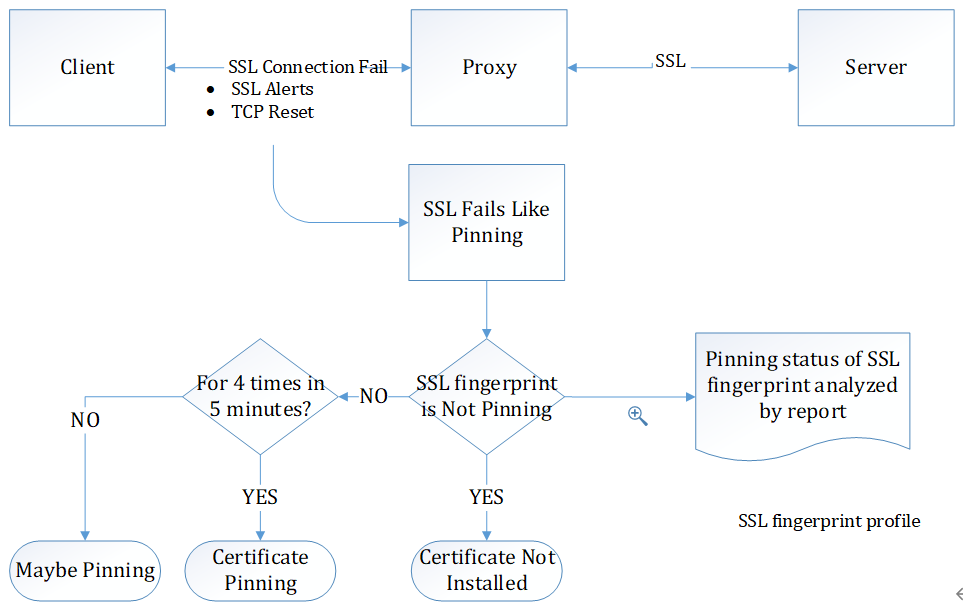
\includegraphics[width=\textwidth]{gfx/dynamic_bypass}
	%\caption{Figure: Inspection Stage}
	\label{fig:system:dynamic_bypass}
\end{figure}

You can configure SSL Proxy to automatically bypass those applications, or alternatively, still intercept to make the client install the trusted root certificate.


Let’s dig into the technical details by a use case. There are two clients, client A and B, reside in our network. They shared a same IPv4 address (NAT), where client A has trusted root certificate installed and uses Facebook app (pinning); client B has no root certificate installed and uses Chrome to visit Facebook website (not pinning). With dynamic bypass configuration:


• Certificate Pinning: Enabled


• Certificate Not Installed: Disabled


At the beginning, both Client A and B’s SSL connections are failed for their own reasons. And then, the proxy identifies client B’s SSL connection as MITMable by finding Chrome’s SSL fingerprints status is Not Pinning in the SSL fingerprint profile. Finally, Client A is bypassed, and client B is not.

\pdfbookmark[3]{Protocol Version}{Protocol Version}
\subsubsection*{\hypertarget{link:Protocol Version}{Protocol Version}}
\label{sec:decrypt:profile:decryptionprofile:version}

Protocol Versions allows you to configure SSL/TLS versions. By default, Proxy mirrors the client versions. Note that some website disable SSLv3 supports for security concerns, set both minimum and maximum version to SSLv3 will interrupt communications. 


HTTP/2 is a major revision of the HTTP network protocol that provide increased speed. If Allow HTTP/2 is enabled, user will have better experience, but requires third-party systems to be able to process decrypted HTTP/2 traffic.

\pdfbookmark[3]{Create a Decryption Profile}{Create a Decryption Profile}
\subsubsection*{\hypertarget{link:Create a Decryption Profile}{Create a Decryption Profile}}
\label{sec:decrypt:profile:decryptionprofile:create}

Perform the following to create a decryption profile:

\begin{description}
    \item[STEP 1.]	Select \textbf{Settings} > \textbf{Proxy Profile}, select \textbf{Decryption Profile} tab, and click \textbf{Create}.
    \item[STEP 2.]	Add a \textbf{Name}. The name is case-sensitive and can have up to 128 characters.
    \item[STEP 3.]	Enable or disable the following certificate checks: \textbf{Common Name}, \textbf{Issuer}, \textbf{Self-signed} and \textbf{Expiry Date}. If you enable Common Name, select Fail-close or Pass-through as your \textbf{Fail Action}. 
    \item[STEP 4.]	Enable or disable the following Dynamic bypass: \textbf{EV Certificate}, \textbf{Certificate Transparency}, \textbf{Mutual Authentication}, \textbf{On Protocol Errors}, \textbf{Certificate Pinning}, \textbf{Certificate Not Installed}.
    \item[STEP 5.]	Enable or disable the following Protocol Versions: \textbf{Mirrors Client Versions}, \textbf{Allow HTTP/2}. If you disable Mirrors Client Versions, you need to select the Min Version and Max Version from SSLv3.0, TLSv1.0, TLSv1.1, TLSv1.2 and TLSv1.3. 
\end{description} 

Go back to Decryption Profile tab, you can view detailed information about the profile you just created. To edit and delete, find the item you want to edit or delete in the list. 
Click \textbf{Edit} or \textbf{Delete} at the top left. You can search profile list based on ID and Name. Enter search conditions in search bar and click search icon.
